\documentclass[12pt,a4paper]{report}
\usepackage[utf8]{inputenc}
\usepackage[francais]{babel}
\usepackage[T1]{fontenc}
\usepackage{amsmath}
\usepackage{amsfonts}
\usepackage{amssymb}
\usepackage{graphicx}
\usepackage{url}
\usepackage{hyperref}
\usepackage[left=2cm,right=2cm,top=2cm,bottom=2cm]{geometry}
\usepackage{listings}
\usepackage{color}

\hypersetup{
backref=true, %permet d'ajouter des liens dans...
pagebackref=true, %...les bibliographies
hyperindex=true, %ajoute des liens dans les index.
colorlinks=true, %colorise les liens
breaklinks=true, %permet le retour à la ligne dans les liens trop longs
urlcolor=red, %couleur des hyperliens
linkcolor=blue, %couleur des liens internes
bookmarks=true, %créé des signets pour Acrobat
bookmarksopen=true, %si les signets Acrobat sont créés,
					%les afficher complètement.
pdftitle={Laboratoire de transmission de signal}, %informations apparaissant dans
pdfauthor={DESSANDE Alexandre, DETOURNAY Jérôme,PECRIAUX Thomas, WERY Michael}, %dans les informations du document
pdfsubject={Fonctionnement du projet} %sous Acrobat.
}

\author{\href{mailto:alex.4492@gmail.com}{Dessandé Alexandre},\href{mailto:jeje.det@gmail.com}{Detournay Jérôme}, \href{mailto:pecriaux.thomas.01@henallux.be}{Pecriaux Thomas}, \href{mailto:wery.michael@gmail.com}{Wery Michael}}
\title{\texttt{\textbf{Laboratoire de transmission de données : \\Manuel d'utilisateur}}}

\begin{document}

\definecolor{mygray}{rgb}{0.5,0.5,0.5}

\lstset{
	backgroundcolor=\color{white},   % choose the background color; you must add \usepackage{color} or \usepackage{xcolor}
	basicstyle=\ttfamily,        % the size of the fonts that are used for the code
	breakatwhitespace=false,         % sets if automatic breaks should only happen at whitespace
	breaklines=true,                 % sets automatic line breaking
%	captionpos=b,                    % sets the caption-position to bottom
	commentstyle=\color{green},      % comment style
	deletekeywords={...},            % if you want to delete keywords from the given language
	escapeinside={\%*}{*)},          % if you want to add LaTeX within your code
%	extendedchars=true,              % lets you use non-ASCII characters; for 8-bits encodings only, does not work with UTF-8
	frame=single,                     % adds a frame around the code : single, lines
	keepspaces=true,                 % keeps spaces in text, useful for keeping indentation of code (possibly needs columns=flexible)
	keywordstyle=\color{blue},       % keyword style
	language=C,		                 % the language of the code
	morekeywords={*,...},            % if you want to add more keywords to the set
	numbers=left,                    % where to put the line-numbers; possible values are (none, left, right)
	numbersep=10pt,                  % how far the line-numbers are from the code
	numberstyle=\tiny\color{mygray}, % the style that is used for the line-numbers
	rulecolor=\color{black},         % if not set, the frame-color may be changed on line-breaks within not-black text (e.g. comments (green here))
	showspaces=false,                % show spaces everywhere adding particular underscores; it overrides 'showstringspaces'
	showstringspaces=true,           % underline spaces within strings only
	showtabs=false,                  % show tabs within strings adding particular underscores
	stepnumber=2,                    % the step between two line-numbers. If it's 1, each line will be numbered
	stringstyle=\color{red},         % string literal style
	morecomment=[l][\color{magenta}]{\#},
	tabsize=2,                       % sets default tabsize to 2 spaces
%	title=\lstname                   % show the filename of files included with \lstinputlisting; also try caption instead of title
literate=
  {á}{{\'a}}1 {é}{{\'e}}1 {í}{{\'i}}1 {ó}{{\'o}}1 {ú}{{\'u}}1
  {Á}{{\'A}}1 {É}{{\'E}}1 {Í}{{\'I}}1 {Ó}{{\'O}}1 {Ú}{{\'U}}1
  {à}{{\`a}}1 {è}{{\'e}}1 {ì}{{\`i}}1 {ò}{{\`o}}1 {ò}{{\`u}}1
  {À}{{\`A}}1 {È}{{\'E}}1 {Ì}{{\`I}}1 {Ò}{{\`O}}1 {Ò}{{\`U}}1
  {ä}{{\"a}}1 {ë}{{\"e}}1 {ï}{{\"i}}1 {ö}{{\"o}}1 {ü}{{\"u}}1
  {Ä}{{\"A}}1 {Ë}{{\"E}}1 {Ï}{{\"I}}1 {Ö}{{\"O}}1 {Ü}{{\"U}}1
  {â}{{\^a}}1 {ê}{{\^e}}1 {î}{{\^i}}1 {ô}{{\^o}}1 {û}{{\^u}}1
  {Â}{{\^A}}1 {Ê}{{\^E}}1 {Î}{{\^I}}1 {Ô}{{\^O}}1 {Û}{{\^U}}1
  {œ}{{\oe}}1 {Œ}{{\OE}}1 {æ}{{\ae}}1 {Æ}{{\AE}}1 {ß}{{\ss}}1
  {ç}{{\c c}}1 {Ç}{{\c C}}1 {ø}{{\o}}1 {å}{{\r a}}1 {Å}{{\r A}}1
  {€}{{\EUR}}1 {£}{{\pounds}}1
}
\maketitle
\setcounter{tocdepth}{4}
\tableofcontents

\chapter{Introduction}
	\section{Matériels et logiciels nécessaires}
	\renewcommand {\labelitemii }{$\diamond $}	
		\begin{itemize}
			\item Matériels			
			\begin{itemize}
				\item Une carte électronique réalisé lors de la deuxième TI IESN		
				\item Un câble usb : A utiliser en simulation de port com		
				\item Un module RFID
				\item Des cartes à puce RFID
				\item Un câble Ethernet : Pour la connexion tcp/ip
			\end{itemize}
			\item logiciels
			\begin{itemize}
				\item Logiciel en \verb+C+ à mettre sur le système embarqué
				\item serial Bootloader AN1310 : Pour écrire le logiciel \verb+C+ sur la carte
				\item Programme en \verb+C#+ donné
			\end{itemize}
		\end{itemize}
	\section{Installation du logiciel C sur la carte}
	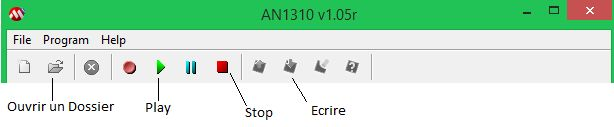
\includegraphics[scale=0.6]{BootloaderBouton.jpg}
		\begin{enumerate}
			\item Connecter la carte en usb au pc
			\item Ouvrir le serial Bootloader AN131
			\item Choisir dans setting le bon port com et mettre le Baud Rate à 9600
			\item Appuyer sur le bouton reset de votre et carte et de suite après sur le bouton de fermeture du programme Bootloader
			\item Ouvrez le fichier \verb+.hex+ et écrivez le
			\item Lancez le programme et fermé la fenêtre du logiciel Bootloader
			\item Bravo le logiciel est installé :)
		\end{enumerate}

\chapter{Utilisation du logiciel C\#}
	\section{Configuration de vos paramètres ip local}
		\begin{itemize}
			\item IP : 10.101.11.102
			\item Masque : 255.255.255.0
		\end{itemize}
	\section{Démarrage}
		\begin{enumerate}
			\item Lancez le programme \verb+.exe+
			\item Passer votre carte à puce sur le module RFID et appuyez sur le bouton central
			\item L'id d'utilisateur s'affiche sur le LCD 
			\item Vous devez maintenant être authentifiez 
			\item Toutes les données devraient se mettre à jour automatiquement
		\end{enumerate}
		Problème pouvant intervenir : 
		\begin{enumerate}
			\item Carte non détecté : Un message apparait sur le LCD "Pas de carte". Veuillez recommencer l'opération.
			\item Utilisateur sans droit : Si vous n'avez pas droit à l'accès un message s'affichera à l'écran de l'ordinateur. Les utilisateurs par défauts en autorisés sont "TOTO, TATA, TITI".
		\end{enumerate}
		
	\section{Utilisation du logiciel}
		\subsection{Ping}
			Vous avez l'occasion grâce au bouton ping de pouvoir vérifier la connectivité avec la carte. 
		\subsection{Mise de donner sur la carte à puce RFID}
			Dans la box formulaire vous pouvez mettre un ID et l'envoyer sur la carte préalablement mise sur le module RFID. Si l'écriture ce passe bien, il sera mis sur le LCD "écriture ok".
		\subsection{Données visibles}
			Le logiciel vous permet de voir différents paramètre :
			\begin{itemize}
			\item La température ambiante
			\item La luminosité
			\item L'IP du système embarqué
			\item L'ID de l'utilisateur connecté.
			\end{itemize}
			
	

\end{document}